% Chapter Deployment
\chapter{Deployment on AWS}
This chapter discusses server farm assembly for running whirlpool on a on-demand resources offered by
AWS. It uses altitude analogy to illustrate important additions in infrastructure at various levels in
detail.

\section{Infrastructure from 10,000 feet}\label{infra10k}
Given a working knowledge of AWS and a crawler which is replicated on to more than one machine, it 
becomes naturally obvious to setup a subnet within a Virtual Private Cloud(VPC) and launch EC2 instances
in it. The subnet within a VPC belongs to single Availability Zone(AZ). 
\begin{figure}[h!]
  \centering
  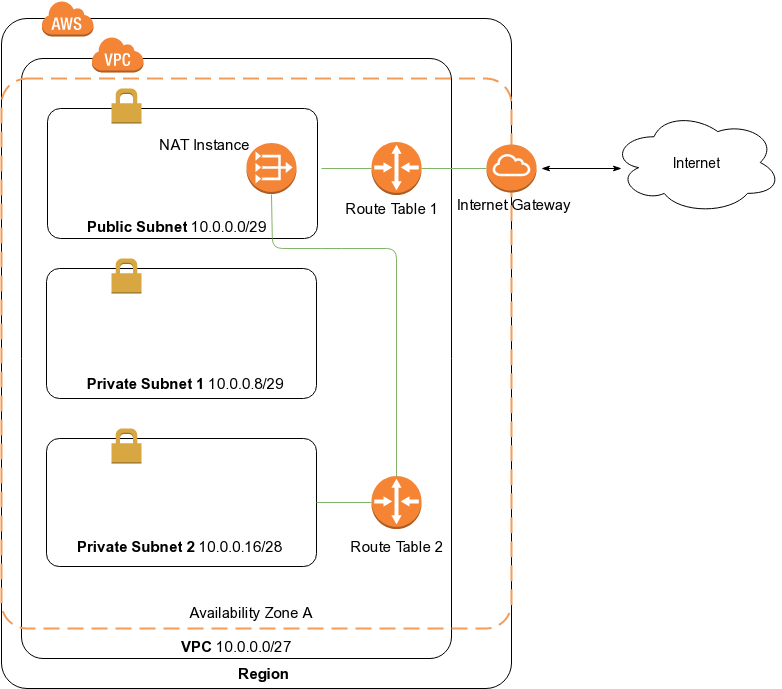
\includegraphics[width=18cm,height=12cm,keepaspectratio]{../media/crawler/ten-thousand-feet-aws.png}
  \caption{Whirlpool Infrastructure using VPC, AZ, and subnet sizing}
  \label{fig:infra10k}
\end{figure}

\noindent
Next, the nature of crawling process is such that it will make outgoing connections to the web servers and never except incoming connections which means the subnet should allow outbound traffic and deny inbound traffic. According to the default behavior of AWS VPC, a private subnet is denied any inbound/outbound connections to the internet. To enable access to the internet within a subnet, a Internet Gateway(IGW) is attached to the VPC.
\\
\\
\noindent
Moreover, the subsystems of whirlpool leverage relational database to maintain a history of URLs, NoSQL to
store extracted text which is then used by the presentation tier to render the data to the public. Also,
later on, a cache server can be adopted to optimize lookup efficiency of various components. Given this
requirement, its safer to form a second private subnet dedicated to placement of data stores and a third
subnet which is public to host application server as shown in the figure \ref{fig:infra10k}. This way, the data store subnet would stay safer routing traffic only within the VPC.
\\
\\
\noindent
Figure \ref{fig:infra10k} uses Classless Inter-Domain Routing(CIDR) block of \ipAddress{10.0.0.0/26} which
gives a range of \ipAddress{64} IPv4 addresses. This thesis uses a tool \cite{cidr} to calculate CIDR
blocks. AWS VPC reserves first four and last IPv4 addresses of each subnet created for internal usage and
therefore cannot be assigned to any instance of any resource. The primary CIDR block size of VPC is used
then used to create 3 subnets within the VPC each with a non-overlapping CIDR block size. The minimum
subnet size allowed is \ipAddress{28} and \ipAddress{16}.
\\
\\
CIDR block size is given by $2^{(32 - x)}$, substituting $x$ = 26 yields,
\begin{align*}
  2^{(32 - 26)} &= 64 && \text{IP addresses} \\
\end{align*}
\\
3 subnets formation = $\underbrace{16}_\text{public}$ + $\underbrace{16}_\text{1st private}$ + $\underbrace{32}_\text{2nd private}$
\\
\\
Actual IP addresses available = $\underbrace{11}_\text{public}$ + $\underbrace{11}_\text{1st private}$ + $\underbrace{27}_\text{2nd private}$
\\
\\
Public subnet IP range = \ipAddress{10.0.0.0/28} $\rightarrow$ (0 - 15)
\\                                                
1st Private subnet IP range = \ipAddress{10.0.0.0/28} $\rightarrow$ (16 - 31)
\\                                                
2nd Private subnet IP range = \ipAddress{10.0.0.0/28} $\rightarrow$ (32 - 64)